\documentclass[11pt]{article}
\usepackage{amsmath,amssymb}
\usepackage{tikz}
\usetikzlibrary{calc}

% Define colors
\definecolor{myblue}{RGB}{0, 75, 243}
\definecolor{myred}{RGB}{255, 0, 0}
\definecolor{mybrown}{RGB}{165, 42, 42}

\begin{document}

\begin{center}
    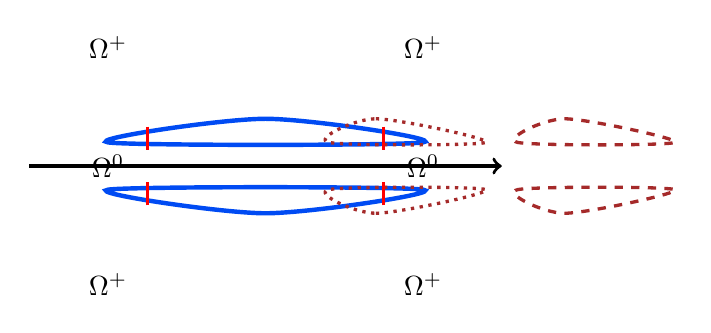
\begin{tikzpicture}[scale=1]
        \draw[->, very thick] (-3,0) -- (3,0);
        \node[] at (-2,0) {$\Omega^0$};
        \node[] at (2,0) {$\Omega^0$};
        \node[] at (-2,-1.5) {$\Omega^+$};
        \node[] at (2,-1.5) {$\Omega^+$};
        \node[] at (-2,1.5) {$\Omega^+$};
        \node[] at (2,1.5) {$\Omega^+$};

        \draw[myblue, ultra thick] 
            plot [smooth cycle] coordinates {(-2,0.3) (0,0.6) (2,0.3)}
            plot [smooth cycle] coordinates {(-2,-0.3) (0,-0.6) (2,-0.3)};

        \draw[mybrown, dashed, very thick] 
            plot [smooth cycle] coordinates {(3.2,0.3) (3.8,0.6) (5.2,0.3)}
            plot [smooth cycle] coordinates {(3.2,-0.3) (3.8,-0.6) (5.2,-0.3)};

        \draw[mybrown, dotted, very thick] 
            plot [smooth cycle] coordinates {(0.8,0.3) (1.4,0.6) (2.8,0.3)}
            plot [smooth cycle] coordinates {(0.8,-0.3) (1.4,-0.6) (2.8,-0.3)};

        \draw[myred, very thick] (-1.5,0.5) -- (-1.5,0.2);
        \draw[myred, very thick] (1.5,0.5) -- (1.5,0.2);

        \draw[myred, very thick] (-1.5,-0.5) -- (-1.5,-0.2);
        \draw[myred, very thick] (1.5,-0.5) -- (1.5,-0.2);
    \end{tikzpicture}
\end{center}

Examples of singular free boundary points where the function $u - \psi$ has strict quadratic growth. We expect quadratic growth in the direction of the \textcolor{myred}{red} arrows. The case on the right is more degenerate than the case on the left, and worse for the approximation of the free boundary $\Gamma$ (depicted in \textcolor{myblue}{blue}). In both cases we have that $\dim \ker \mathbf{A} = 1$. A discrete free boundary $\Gamma_{\Delta}$, which is at a distance $\mathcal{O}(\delta(h)^{1/2})$ is depicted in \textcolor{mybrown}{dashed brown}.

\end{document}